%*****************************************
\chapter{Automatic Speech Recognition}\label{ch:speech-recognition}
%*****************************************

\section{The big picture}

Basically, all statistical methods of \ac{ASR} are dedicated into solving one fundamental 
equation, which can be described as follows. Let $O$ be a sequence of observable acoustic 
feature vectors and $W$ be a word sequence, the most likely word sequence $W*$ is given by:

\begin{equation}{\label{eq:fund-asr}}
W*= \arg\max_{W}P(W|O)
\end{equation}

To solve this equation straightforwadly, one would require a discriminative model,
capable of estimating the the probability of $W$ directly from a set of observations $O$ \cite{Gales2007}.
However, \ac{HMM} are generative models and are not adequate for solving this equation,
therefore we apply Bayes' Theorem to Equation~\ref{eq:fund-asr} and end up with:

\begin{equation}
W*= \arg\max_{W}\frac{P(O|W)P(W)}{P(O)}
\end{equation}

As one might notice, we can apply a generative model to calculate the conditional probability term of this
equation, that is, the probability of the observation sequence $O$ given a word sequence $W$, hence $P(O|W)$.
At first, it might seem counter-intuitive to conceive a generative model for data analysis, since the 
data is already available, i.e. $O$ is known before-hand. As \citeauthor{Fink2008}~\citep{Fink2008} points 
outs, in order to understand how to generative models are used for data analysis, a mental trick is necessary.

[To fix - Fink citation]First one assumes, that the data
to be analyzed were generated by a natural process, which obeys similar statistical
regularities. Then one tries to reproduce this process with the capabilities of hidden
Markov models as closely as possible. If this attempt is successful, on the basis of
the artificial model inferences can be drawn on the real process. On the one hand
this may concern the probability for generating the available data. On the other hand
the inference on the internal processes within the model is at least probabilistically
possible. In particular one can determine the state sequence that generated a certain
sequence of outputs with highest probability.

For a single audio input, which we want to decode, the audio is already fixed, so the 
probability of the observable acoustic feature vectors $P(O)$ is a constant and, therefore, 
might be discarded. Thus the final fundamental equation is simplified to:

\begin{equation}
W*= \arg\max_{W}P(O|W)P(W)
\end{equation}

$P(O|W)$, the probability of an observable acoustic feature vector given a word sequence, is calculated by 
an acoustic model. In turn, $P(W)$, the \emph{a priori} probability of words is reckoned by a language model.

\section{HMM}

Markov models consist a set of mathematical models which are suitable for the statistical description of symbol
and state sequences \cite{Fink2008}. The simplest form of Markov models are Markov chain models, 
which represent a system with a set of spaces in which transitions from one state to another occur. 
Within Markov processes, systems are assumed to be memoryless, that is, the conditional probability
of future states is only dependent on the present state. To put it another way, Markov models assume that,
given a certain system with states and transitions, the current state does not depend upon the 
sequence of events that preceded it, the so-called Markov property. 

\ac{HMM}s can be formally described as a 5-tuple $\lambda = \left (Q, O, \Pi, A, B\right )$, where $Q = \left \{q_1, q_2, q_3, ..., q_N\right \}$  is a set of $N$ states. $O = \left \{o_1, o_2, o_3, ..., o_T\right \}$ is a set of $T$ observations taken from time $t = 1$ to $t = T$. At each time $t$ it is assumed that the system will be at a specific state $q$, which is hidden, only the observations are directly visible. $\Pi = \left \{\pi_i \right \}$ is a vector with the initial state probabilities, such that
\begin{equation}
\pi_i = Pr(q_i), t = 0
\end{equation}
$A = [a_{ij}]$ is matrix with the state transition probabilities so that
\begin{equation}
a_{ij} = P(q_t = j | q_{t-1} = i),  1 \leq, i, j \leq N
\end{equation}
and $B = [b_{jt}]$ is a matrix with the emission probability of each state. Assuming a \ac{GMM} to model the state emission probabilities -- the so-called GMM/HMM model; we can define that, for a state $j$, the probability $b_j(o_t)$ of generating $o_t$ is given by
\begin{equation}
 b_j(o_t) = \prod_{s=1}^{S}\left [ \sum_{m=1}^{M_{js}} c_{jsm}\mathcal{N}(o_{st}; \mu_{jsm}, \Sigma_{jsm}) \right ]^{\gamma_s}
\end{equation}
where $\gamma s$ is a stream weight, with default value is one, $M_{js}$ is the number of mixture components in state $j$ for stream $s$, $c_{jsm}$ is the weight of the $m$\textsuperscript{th} component and $\mathcal{N}(\cdot; \mu_{jsm}, \Sigma_{jsm})$ is a multivariate Gaussian with mean vector $\mu$ and covariance matrix $\Sigma$, that is
\begin{equation}
 \mathcal{N}(o; \mu, \Sigma) = (\sqrt{(2\pi)^{n}\left |\Sigma\right |})^{-e^{-\frac{1}{2}(o-\mu)^{T}\Sigma^{-1}(o-\mu)}}
\end{equation}
where $n$ is the dimensionality of $o$.

The following constraints apply:
\begin{equation}
a_{ij} \geq 0
\end{equation}
that is, the probability of moving from state from any state $i$ to $j$ is not null, and
\begin{equation}
\sum_{j=1}^{N} a_{ij} \geq 1, \forall i
\end{equation}

\section{PB}
15 Reconhecimento Autom\'atico de Fala (RAF)

O prop\'osito de um reconhecedor de fala \'e transformar, de forma eficiente
e precisa, o sinal ac\'ustico da fala em sua contraparte textual (Rabiner
\& Schafer, 2007). Se cada palavra da l\'ingua fosse pronunciada de forma
id\^entica por todos os falantes e em todos os contextos, a tarefa de
Reconhecimento Autom\'atico de Fala (doravante RAF) seria algo banal. Mas
isso n\~ao acontece: a realidade lingu\'istica \'e demasiado variante, quer
inter- , quer intrafalantes. Pode-se, por fim, dizer que uma vogal nunca
\'e pronunciada de uma mesma maneira. Furui (2001) sumariza os problemas
do RAF em quatro: (i) dificuldades em lidar com coarticula\c{c}\~ao e redu\c{c}\~ao;
(ii) dificuldades de segmenta\c{c}\~ao da fala; (iii) diferen\c{c}as
inter-individuais; e (iv) insufici\^encia de conhecimento lingu\'istico. A
seguir, cada um desses pontos ser\~ao discutidos.

A coarticula\c{c}\~ao \'e um  fen\^omeno  motor  que  envolve  a  realiza\c{c}\~ao  de
gestos articulat\'orios simult\^aneos ou sobrepostos (Crystal, 2008). Na
fala, a coarticula\c{c}\~ao pode ocorrer de duas formas: antecipat\'oria
(left-to-right) ou preservativa (right-to-left). Na coarticula\c{c}\~ao
antecipat\'oria, um som \'e realizado tomando as caracter\'isticas de outro
que lhe sucede. Em ``pulo'', por exemplo, a consoante /p/ \'e realizada
com protrus\~ao labial, {[}p?{]}, em virtude de a vogal que lhe segue,
{[}u{]}, ser arredondada. Por sua vez, na coarticula\c{c}\~ao preservativa, um
som \'e realizado mantendo-se as caracter\'isticas articulat\'orias de outro
que lhe antecede. Em dialetos em que n\~ao houve a vocaliza\c{c}\~ao da lateral,
por exemplo, a consoante /l/ da palavra ``sal'' pode ser realizada de
modo velarizado, {[}?{]} em vez de {[}l{]}, por suceder a vogal {[}a{]},
que \'e baixa. De fato, a todo o tempo, os sons da fala est\~ao sujeitos à
coarticula\c{c}\~ao. Por tal raz\~ao, frequentemente, utilizam-se no RAF
unidades fon\'eticas dependentes de contexto, a exemplo de trifones.

Um trifone \'e uma representa\c{c}\~ao fon\'etica contextual, que considera, para
um dado fone, o fone anterior e o seguinte. A palavra `fala', por
exemplo, pode ser representada, no IPA, pela sequ\^encia de fones
{[}'fal?{]} ou de trifones {[}\#'fa fal al? l?\#{]}, especificando-se as
articula\c{c}\~oes secund\'arias dos fones. No reconhecimento de fala, por
raz\~oes de codifica\c{c}\~ao em computadores, em geral, os trifones s\~ao
especificados no formato ``L-X+R'', em que ``X'' \'e um determinado fone,
``L'' o fone antecedente, e ``R'' o sucessor. A Figura 6 compara a
transcri\c{c}\~ao da palavra ``translate'' em fones e trifones.

                                [pic]

Figura 6: Transcri\c{c}\~ao da palavra ``translate'' em fones e trifones de
acordo com a conven\c{c}\~ao do VoxForge (2013).

Quanto às diferen\c{c}as interindividuais, elas s\~ao tamanhas que h\'a at\'e
mesmo todo um ramo de investiga\c{c}\~ao da Lingu\'istica que se dedica a seu
estudo: a Sociolingu\'istica. A Sociolingu\'istica estabelece que a
realiza\c{c}\~ao lingu\'istica \'e condicionada por diversos fatores sociais: o
n\'ivel escolar do falante, seu sexo, sua idade, seu estrato social, o
lugar onde nasceu e viveu, a situa\c{c}\~ao comunicativa em que est\'a inserido,
a formalidade de registro que o contexto demanda, o grau de hierarquia
que mant\'em com seu interlocutor, etc. (Labov, 2008; Weinreich et al.,
2006). Para al\'em dos fatores que condicionam a varia\c{c}\~ao, h\'a fen\^omenos
lingu\'isticos que possuem comportamento puramente estoc\'astico: o
al\c{c}amento voc\'alico acontece em certas vezes e n\~ao em outras, mesmo
havendo o mesmo ambiente e considerando- se o mesmo falante.

N\~ao bastassem os fatores sociais, a fala sofre influ\^encia tamb\'em de
caracter\'isticas anat\^omicas do indiv\'iduo. A variabilidade lingu\'istica
come\c{c}a j\'a quando somos crian\c{c}as, na fase de desenvolvimento puberal. Das
primeiras palavras que balbuciamos at\'e o per\'iodo de muda vocal, ocorrem
grandes mudan\c{c}as na voz tendo em vista, especialmente, modifica\c{c}\~oes nas
configura\c{c}\~oes das estruturas lar\'ingeas (Guimar\~aes, 2006). Perry et al.
(2001) conduziram um estudo sobre vogais produzidas por crian\c{c}as dos 2
aos 16 anos e verificaram que h\'a diferen\c{c}as significativas nos valores
de frequ\^encia fundamental {[}pic{]} e nos formantes das vogais
{[}pic{]}. Ao longo de todo o per\'iodo de matura\c{c}\~ao de voz, os valores de
frequ\^encia dos formantes das vogais {[}pic{]} varia significativamente e
\'e distinto para meninos e meninas; ap\'os os 12 anos, h\'a grande decr\'escimo
nos valores de frequ\^encia fundamental {[}pic{]} para os meninos, de modo
que a frequ\^encia fundamental {[}pic{]} passa tamb\'em a servir
perceptualmente para a distin\c{c}\~ao do sexo das crian\c{c}as (Perry et al.,
2001) (Figura 7).

                                [pic]

Figura 7: Compara\c{c}\~ao dos valores de ??0, F1, F2 e F3 para crian\c{c}as de
ambos os sexos dos 2 aos 16 anos (Perry et al., 2001).

Aos sistemas de RAF, cabe a tarefa de reconhecer, ante toda a
variabilidade lingu\'istica existente, o que h\'a de invariante na fala. Do
ponto de vista computacional, a constru\c{c}\~ao de um reconhecedor de fala
pode ser vista como uma tarefa que abrange quatro fases principais:
prepara\c{c}\~ao de dados, treino, teste e an\'alise (Young, et al., 2006). A
prepara\c{c}\~ao de dados consiste na grava\c{c}\~ao de arquivos de \'audio e texto,
em sua anota\c{c}\~ao, transcri\c{c}\~ao e pr\'e-processamento, de modo a garantir que
a entrada seja compat\'ivel com o esperado pelo reconhecedor. O treino
constitui a fase em que os dados coligidos s\~ao utilizados para criar as
componentes do reconhecedor. Em geral, os sistemas de RAF possuem tr\^es
componentes: (i) um modelo de l\'ingua, (ii) um modelo ac\'ustico e (iii) um
modelo de pron\'uncia, ou dicion\'ario de pron\'uncia. Por fim, as fases de
teste e an\'alise buscam verificar se os modelos constru\'idos se ad\'equam à
realidade lingu\'istica ou ao prop\'osito a que o reconhecedor se disp\~oe.

16 Representa\c{c}\~ao Digital da Fala

Para desenvolver tecnologias de fala, \'e preciso antes encontrar formas
de codificar, computacionalmente, a informa\c{c}\~ao presente na fala. A fala
humana, como constitui um ve\'iculo de informa\c{c}\~ao, pode ser vista a partir
de uma perspectiva da Teoria Matem\'atica da Comunica\c{c}\~ao (Shannon,
1948){[}11{]}, sendo considerada um sinal ac\'ustico. Tecnicamente, sinais
s\~ao sequencias de estados em um sistema de comunica\c{c}\~ao que codificam uma
mensagem.

Sinais constituem o objeto central de estudo da \'area de Processamento de
Sinal, que busca investigar formas de analisar ou modificar os sinais,
no intuito de deles extrair informa\c{c}\~ao ou de adequ\'a-los a um determinado
fim (Ingle e Proakis, 2011{[}12{]}). Embora a maior parte dos sinais que
nos rodeia seja anal\'ogica, em muitas vezes, seu processamento \'e feito
n\~ao de forma anal\'ogica, mas digital. De acordo com Ingle e Proakis
(2011){[}13{]}, os sistemas de Processamento de Sinal Digital (DSP) s\~ao
vantajosos, pois:

n\~ao necessitam a aquisi\c{c}\~ao de equipamento espec\'ifico (que s\~ao, muitas
das vezes, caros), podendo ser desenvolvidos em computadores pessoais;

baseiam-se apenas em opera\c{c}\~oes num\'ericas de adi\c{c}\~ao e multiplica\c{c}\~ao, o
que lhes d\'a estabilidade, n\~ao sendo necess\'ario calibragem ou
padroniza\c{c}\~ao, como \'e comum nos sistemas anal\'ogicos;

s\~ao altamente adapt\'aveis, de modo que suas opera\c{c}\~oes podem ser
modificadas em tempo real, usualmente, atrav\'es de t\'ecnicas de
programa\c{c}\~ao simples.

Um esquema de um sistema de processamento de sinal digital \'e apresentado
na Figura 8.

                                [pic]

Figura 8: Esquema de um sistema de processamento de sinal digital (Ingle
e Proakis, 2011).

Embora a maior parte dos sinais do mundo seja anal\'ogica - entre os quais
a fala, seu processamento, muitas vezes, d\'a-se gere sinais anal\'ogicos,

Embora a maior parte dos sinais com que

O processamento de sinais pode ser feito de forma anal\'ogica ou digital.

A \'area do conhecimento respons\'avel por tal busca \'e o Processamento de
Sinal.

A \'area respons\'avel por esse

Do ponto de vista da Teoria da Informa\c{c}\~ao, sinais s\~ao sequencias de
estados em um sistema de comunica\c{c}\~ao que codificam uma mensagem.

(Ingle e Proakis, 2010)

17 Tipos de Reconhecedores de Fala

Reconhecedores Autom\'aticos de Fala podem ser agrupados em tr\^es
categoriais, que se dividem quanto à tarefa de reconhecimento que
desempenham: i) reconhecimento de palavras isoladas; ii) de senten\c{c}as
pr\'e-estabelecidas; iii) reconhecimento de fala cont\'inuo de grande
vocabul\'ario (RFCGV){[}14{]} (Rabiner, 1997).

Os sistemas de reconhecimento de palavras isoladas s\~ao utilizados, por
exemplo, por centrais telef\^onicas, nas Unidades de Resposta Aud\'ivel
(URA), em menus do tipo: ``Fale `um' para ser redirecionado ao setor de
cancelamento'' ou ``Para conversar com um de nossos atendentes, fale
`atendente'\,''. Reconhecedores de fala do segundo tipo s\~ao mais
robustos que os do segundo, sendo capazes de reconhecer senten\c{c}as
pr\'e-definidas ou provenientes de uma gram\'atica pr\'e-estabelecida. Um
exemplo de aplica\c{c}\~ao deste tipo s\~ao os m\'odulos de comando por voz de
computadores, celulares e os sistemas hands-free em carros, em que se
pode dizer senten\c{c}as do tipo ``ligar o r\'adio'' ou ``Siri, google `speech
recnognition'\,''e o comando \'e reconhecido. J\'a os sistemas de
reconhecimento de fala cont\'inuo de grande vocabul\'ario s\~ao os
reconhecedores mais abrangentes, sendo capazes de processar a fala
espont\^anea do usu\'ario. Sistemas de di\'alogo por voz, como os How May I
Help You (HMIHY), e sistemas de ditado em editores de textos s\~ao desse
\'ultimo tipo.

A seguir, ser\'a discutida apenas a arquitetura dos sistemas de RFCGV,
primeiro, porque consistem nos sistemas de reconhecimento com a
arquitetura mais complexa e, segundo, porque \'e o tipo de reconhecedor
que se pretende desenvolver neste projeto.

18 Arquitetura B\'asica de um Reconhecedor de Fala Cont\'inuo de Grande
Vocabul\'ario (RFCGV)

O paradigma majorit\'ario em sistemas de RAF \'e estoc\'astico, destacando-se,
especialmente, a utiliza\c{c}\~ao de Modelos Ocultos de Markov, ou Hidden
Markov Models (HMM) (Huang, et al., 2001). Em tais modelos, a tarefa de
reconhecimento \'e considerada a partir da met\'afora do canal ruidoso, ou
noisy-channel (Jurafsky \& Martin, 2009). O sinal ac\'ustico, que
constitui a entrada no sistema, \'e visto como uma deforma\c{c}\~ao da mensagem
original, isto \'e, da sequ\^encia de palavras pretendida pelo falante, ap\'os
passar por um canal com ru\'ido. Assim, o reconhecimento se torna uma
tarefa de decodifica\c{c}\~ao, isto \'e, trata de como recuperar a mensagem
original a partir do sinal ac\'ustico ``ruidoso''. Matematicamente, isso
corresponde a estimar, considerando-se uma l\'ingua {[}pic{]}, para uma
sequ\^encia de palavras {[}pic{]}, qual \'e a sequ\^encia {[}pic{]} mais
prov\'avel, dado conjunto de estados ac\'usticos observ\'aveis {[}pic{]}:

{[}pic{]}

Todavia, n\~ao \'e poss\'ivel calcular {[}pic{]} diretamente, sendo necess\'ario
aplicar-se o Teorema de Bayes, de modo a obter-se:

{[}pic{]}

Como a prop\'osito \'e buscar a sequ\^encia de palavras mais prov\'avel para um
conjunto j\'a dado de estados ac\'usticos, {[}pic{]} se repete a cada
c\'alculo, de maneira que pode ser considerado uma constante de
normaliza\c{c}\~ao, e a equa\c{c}\~ao pode ser simplificada para:

{[}pic{]}

Essa equa\c{c}\~ao fundamenta a base dos sistemas de RAF estoc\'asticos e possui
estreita rela\c{c}\~ao com a arquitetura que \'e por eles compartilhada.
Basicamente, os sistemas de RAF cont\'inuo com grande vocabul\'ario possuem
tr\^es m\'odulos: (i) um modelo de l\'ingua, (ii) um modelo ac\'ustico e (iii)
um modelo, ou dicion\'ario de pron\'uncia. O modelo de l\'ingua \'e utilizado
para estimar {[}pic{]}, a probabilidade a priori da sequ\^encia de
palavras. J\'a o modelo ac\'ustico \'e utilizado para calcular {[}pic{]}, a
verossimilhan\c{c}a da observa\c{c}\~ao. Por fim, o dicion\'ario de pron\'uncia serve
como uma ponte entre o modelo de l\'ingua e o modelo ac\'ustico, uma vez que
possui as palavras que comp\~oem o l\'exico do reconhecedor, transcritas em
forma ortogr\'afica e fon\'etica. A Figura 9 ilustra a arquitetura b\'asica de
um sistema de RAF.

                                [pic]

 Figura 9: Arquitetura b\'asica de um Reconhecedor Autom\'atico de Fala.

O modelo ac\'ustico processa o sinal ac\'ustico da fala, de modo a inferir
quais s\~ao os segmentos sonoros que a comp\~oem, usualmente, empregando
fones ou trifones. Em reconhecedores de base em HMM, essa tarefa \'e feita
estimando-se os estados ac\'usticos observados mais prov\'aveis, bem como
suas probabilidades de transi\c{c}\~ao. J\'a o modelo de pron\'uncia prov\^e a
correspond\^encia entre sequ\^encias de fones e as palavras da l\'ingua. No
exemplo, tal modelo mapeia a sequ\^encia de fones {[}fal?{]} na palavra
``falo''. O modelo de l\'ingua, por sua vez, estima as ordena\c{c}\~oes de
palavras mais prov\'aveis na l\'ingua.

\section{A Brief History}

Although the task of recognizing words from speech might seem apparently simple beforehand,
(after all humans start doing it with as little as four months! (XXXX INSERT CITATION)),
the issue is actually very complex one. Over the years, many methods have been 
proposed to attempt to solve the problem of speech recognition. However until now no solution has been found and machines are still
a very long way from performing like humans. \autoref{tab:comparison-human-mach} presents a comparison between the performance
of humans and machines in some recognition tasks.

\begin{table}[!ht]
  \caption[Word error rate comparisons between human and machines on similar tasks \citep{Huang2001}.]{Word error rate comparisons between human and machines on similar tasks \citep{Huang2001}.}
  \smallskip
  \centering
  \begin{tabular}{lcrr} \toprule
      \tableheadline{Tasks} & \tableheadline{Voc. size} & \tableheadline{Humans} & \tableheadline{Machines} \\ \midrule
      \small Connected digits & 10 & 0.009\% & 0.720\% \\
      \small Alphabet letters & 26 & 1\% & 5\% \\
      \small Spontaneous telephone \\ speech & 2,000 & 3.8\% & 36.7\% \\
      \small WSJ with clean \\ \small speech & 5,000 & 0.9\% & 4.5\% \\
      \small WSJ with noisy \\ \small speech (10-db SNR) & 5,000 & 1.1\% & 8.6\% \\
      \small Clean speech based \\ \small on trigram sentences & 20,000 & 7.6\% & 4.4\% \\
    \bottomrule
  \end{tabular}
  \label{tab:comparison-human-mach}
\end{table}

As one may observe, humans outperform machines in almost every task, specially the more complex ones. 
Humans' are indeed the topline for the speech recognition task, the uttermost dream of each speech 
scientist alive is to build a system capable of performing similarly to humans. Although this dream is somewhat near
for rather simple tasks like connected digits, for other contexts a long path yet lies ahead. 

Recognizing spontaneous speech is still a huge barrier for machines, as can be seen from the huge difference
in the spontaneous telephone corpus: whereas humans had a WER of $3.8\%$, for machines this rate is up to $36.7\%$.
Such result is mainly due to linguistic variability. Language varies not only among speakers (the so-called 
inter-speaker variability), but also within the same speaker (intra-speaker) \citep{Benzeghiba2007}. 

Considering inter-speaker differences, factors such as gender, age, social, and regional 
origin, health and emotional state might have a huge impact on the speech signal \citep{Benzeghiba2007}.
Sociolinguistics has long known that gender affects language usage, in fact, men and women tend to use different language constructions.
In her seminal paper in the field, \citeauthor{Lakoff1973} \citep{Lakoff1973} found that, in women's speech, strong expressions 
of feeling are avoided, uncertainty is favored, and means of expression in regard to subject-matter deemed ``trivial'' to the 
``real'' world are elaborated. 

Put aside social aspects, men, women and children's speech are also contrasting because of morphological differences
in their vocal tract. Sex and development influence body size, and there is a strong correlation between vocal tract length and body size 
(either height or weight); in addition to this, the relative proportions of men and women's oral and pharyngeal cavity are unlike 
\cite{Fitch1999}. \autoref{fig:vocal-tract-morphology-sex} presents a comparison between height and
vocal tract length for men, women and children. \autoref{fig:vocal-tract-morphology} presents a model of the vocal tract morphology considering
age.

\begin{figure}[H]
        \myfloatalign
        {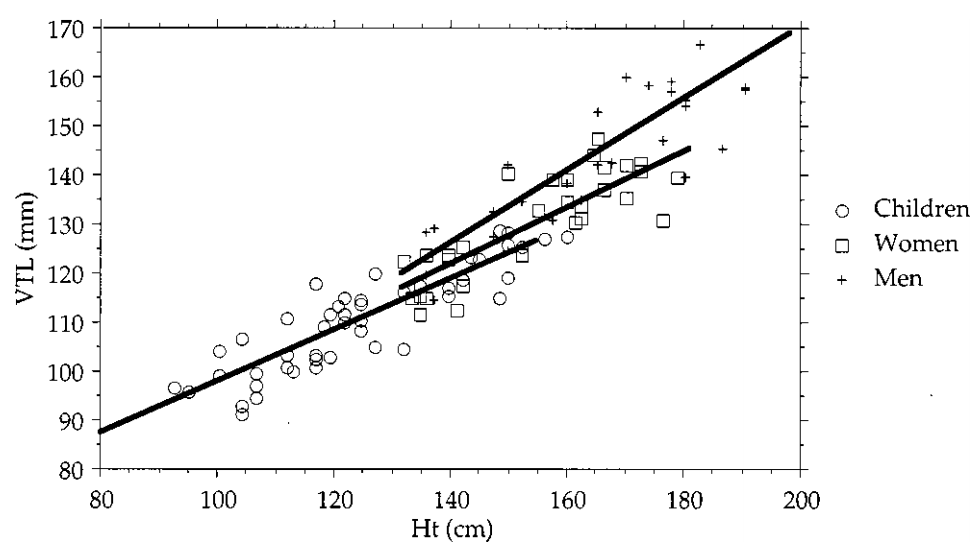
\includegraphics[width=.66\linewidth]{gfx/vocal-tract-size-sex.png}}
        \caption{Height (cm) versus vocal tract length (mm) \cite{Fitch1999}.}
        \label{fig:vocal-tract-morphology-sex}
\end{figure}

\begin{figure}[H]
        \myfloatalign
        {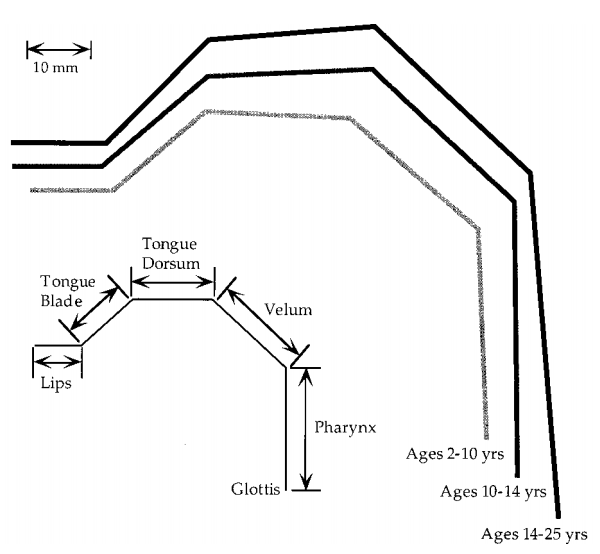
\includegraphics[width=.66\linewidth]{gfx/vocal-tract-size-gender.png}}
        \caption{Averaged vocal tract morphology \cite{Fitch1999}.}
        \label{fig:vocal-tract-morphology}
\end{figure}

As one can observe, men's vocal tract are longer than women's, followed and obviously children. These morphology differences 
affect the speech signal thorougly, specially in what concerns to the \ac{F0}. \ac{F0} can be defined as the 
lowest frequency in the signal counting from zero. \autoref{fig:f0-age-sex} compares the \ac{F0} values
between male and females considering aging.

\begin{figure}[!h]
        \myfloatalign
        {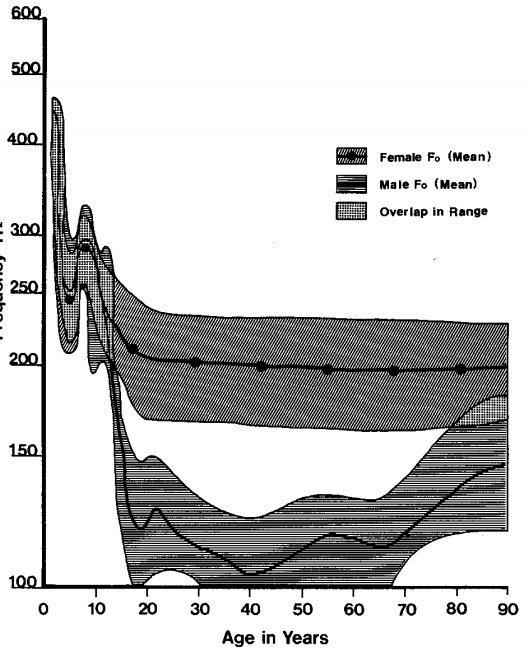
\includegraphics[width=.66\linewidth]{gfx/f0-age-sex.png}}
        \caption{F0 and pitch sigma versus age for males and females \cite{Brown1991}.}
        \label{fig:f0-age-sex}
\end{figure}

One can notice from \autoref{fig:f0-age-sex}, that no difference is found between male and female voice at a very young age. 
In fact, boys and girls have roughly the same \ac{F0} values. However, when they reach puberty, differences begin to appear. 
This period is commonly called the voice mutation or voice change, when the \ac{F0} for male voice has huge drop, while 
for female voice the drop is quite small. In terms of perception, this is period when the male voice lowers and geets deeper.

XXXXXXXXXXXXXXXXXXX EXTEND INTER-SPEAKER VARIABILITY
XXXXXXXXXXXXXXXXXXX DESCRIBE INTRA-SPEAKER VARIABILITY

But let's get back to \autoref{tab:comparison-human-mach}. It is interesting to notice that humans
performed better in all speech recognition tasks, but one: ``Clean speech based on trigram sentences''.
This one task consists of recognizing sentences which were randomly generated using the WSJ trigram language model. 
Therefore, humans had no advantage over machines in what concerns to syntactic or semantic knowledge. 
This result highlights one of the most important feature of human hearing, that is, we make a large use of syntactic, 
semantic and also pragmatic information in order to understand speech. While hearing do not take into account simply 
the acoustic signal, but the whole context. 

Language is a social tool, which aims at successfull interaction. When someone steps into a snack bar and orders 
an [\textipa{aIs"krim}], the vendor has no doubt that this sequence of phones refers to ``ice cream'' and not ``I scream'', 
albeit they are pronounced exactly the same. Although such sequence of phones might be ambiguous in the phonetic level,
it is not in higher linguistic levels, such as syntax (the verb ``order'' is usually followed by a noun), semantics 
(the object of order has to be something purchasable) and pragmatics (one does not buy his own shout!).


\section{HMM-based Speech Recognition} 
\ac{HMM} is the most widespread and successfull paradigm in \ac{ASR}. When \ac{HMM} were first applied
to speech recognition in the late $70$'s, they were completely revoluationary.
Up until recently \ac{DNN} seem to be next prominent paradigm in \ac{ASR}.
\ac{HMM} have been applied
to \ac{ASR} since the late $70$'s, and they have gathered the best results until recently.

A \ac{HMM} is a statistical Markov model in which the states are assumed to be hidden, i.e. they are
not directly visible, only the state's outputs are observable. Each state has a probability distribution 
over the possible output tokens, in such a way that output generated by the HMM states provides some information
about the hidden sequence of states which was traversed.

\section{Feature Extraction}

\subsection{Preambulus}
Feature extraction is an importart part of speech recognition systems. The feacture extraction 
phase is responsible for identifying or enhancing the components of the signal that are relevant 
for recognizing speech sounds, while discarding or diminishing the effect of unuseful information, 
such as background noise. With respect to speech parameterization, \ac{MFCC} are definitely the
standard. \ac{MFCC} have been widely used in \ac{ASR} systems for almost three decades \cite{Davis1980}, 
they are present on the many important speech recognition toolkits, such as \ac{HTK}, Sphinx, \ac{RASR} and Kaldi.
Before we go into further details about these features it is interesting to give a little background 
about speech recording and coding.

Speech is recorded by using a microphone -- nothing new so far!
Despite the many types of available microphones (condenser, capacitor, pyezoeletric, laser, etc.) its design
remains basically the same as the carbon microphone invented by David Hughes two centuries ago \cite{Robjohns2010}.
A microphone is simply an acoustic-to-electric sensor, which converts variations in air pressure (that is, sound)
into an electrical signal. Microphones have a very thin membrane, called diaphragm, which vibrates when struck by 
sound waves.  When the diaphragm vibrates, it puts to move a sensitive capsule attached to it, 
that converts its movement into electrical pulses. Most of the current microphones are dynamic, which means 
that their capsule consist of  .... (XXX VER WIIPEDIA)

After capturing speech through a microphone, one usually wants to store it for later access. In order
to store speech digitally on a computer, a coding scheme is mandatory. In the literature, many coding schemes have
been proposed, such as linear PCM, $\mu$-law, A-law PCM, APCM, DPCM, DM, and ADPCM \cite{Huang2001}. The details of 
each type of speech coder is beyond the scope of this dissertation, the reader can 
find an description of each scheme in \citeauthor{Huang2001} \citep{Huang2001} or \citeauthor{Furui2001} \citep{Furui2001}. 
Following we will give a brief discussion of linear PCM, which is the standard way of storing audios in digital format. 

\ac{PCM} is a type of analog-to-digital conversion, which constitutes the basis of the WAV digital audio format, together
with other lossless formats such as AIF and AU.
\footnote{Other types of popular audio files which use lossy data compression, such as MP3, WMA, OGG or AAC (a format common to 
DivX videos) do not use PCM. Instead}. 
PCM coding is based on two properties: (i) a sampling rate of the audio and a (ii) bit depth. The sampling rate determines the
number of audio samples that are taken per second from the signal, in turn the bit depth is the number of bits 
of information in each audio sample. Both values must be constant and should be defined prior to recording (actually coding) an audio. 
The sampling and the bit depth are closely related to the audio quality, that is, the higher the sampling and the depth
the better the fidelity of the digital audio to the analog speech signal. Picture XXX presents an example of a linear PCM 
representation, at different sampling rates and bit depths, of an audio containing the utterance ``Speech recognition''.

Linear PCM assumes that the discrete signal $x[n]$ is bounded, that is,
\begin{equation}
|x[n]| \leq X_{max} 
\end{equation}
and that the quantization step $\Delta$ is uniform for all consecutive levels of $x_i$
\begin{equation}
x_i - x_{i-1} = \Delta
\end{equation}

Assuming a binary code, the number of levels which can be represented by PCM is $N=2^B$, where $B$ is the bit depth, this constitutes
the audio resolution. According to \citep{Huang2001}, speech could be represented in an intelligible way by using 7 bits, however, in 
practice, applications use values no lower than 11 bits to guarantee communication efficiency. For instance, CDs makes use of 16-bit 
linear PCM, whereas DVD-Audio and Blu-Ray discs can support up to 24-bit.

Although linear PCM files are able to carry all the necessary auditory information -- after all we are able to listen to them and
recognize the speech, the music or the noise recorded in them; they are not useful for speech recognition purposes. This occurs 
because, from the phonological point of view, very little can be said based on the waveform itself \citep{Shrawankar2010}.
Consider, for instance, the two combinations of 100 Hz, 200 Hz and 300 Hz sine waves, shown in \autoref{fig:complex-waves-pure-tones}, 
which differ only with respect to the relative timing.

\begin{figure}[!h]
        \myfloatalign
        {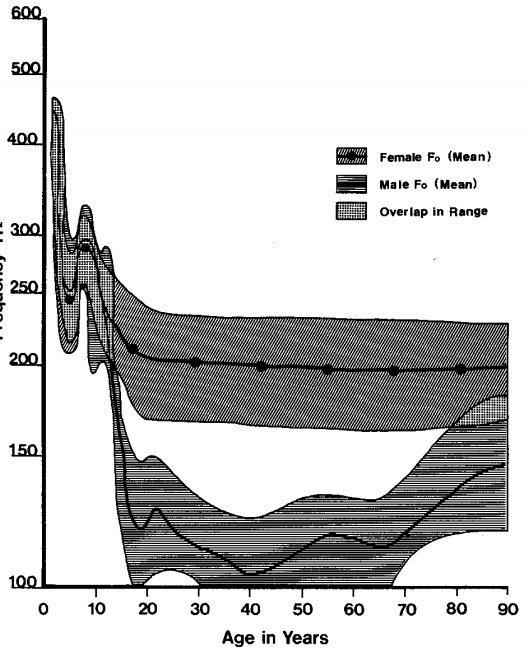
\includegraphics[width=.66\linewidth]{gfx/f0-age-sex.png}}
        \caption{Two complex waveforms generated by the same three pure tone 100 Hz, 200 Hz and 300 Hz sine waves, differing only 
        with respect to their relative timing \cite{Ladefoged1996}.}
        \label{fig:complex-waves-pure-tones}
\end{figure}
 
As one might notice, disregard of being composed by the same pure tones, the complex waves shown in 
\autoref{fig:complex-waves-pure-tones} are completely distinct from one another. This happens because the waveform is influenced
by phase shifts (also known as phase offsets). Therefore in-phase and out-of-phase waves (\autoref{fig:in-phase-waves} and
\autoref{fig:out-of-phase-waves}) are represented differently, and this adds too much variability to the waveform, in such way that
the signal waveform becomes unsuitable for human analysis and consequently for being used as a raw input in \ac{ASR} systems. 


\begin{figure}[!h]
        \myfloatalign
        {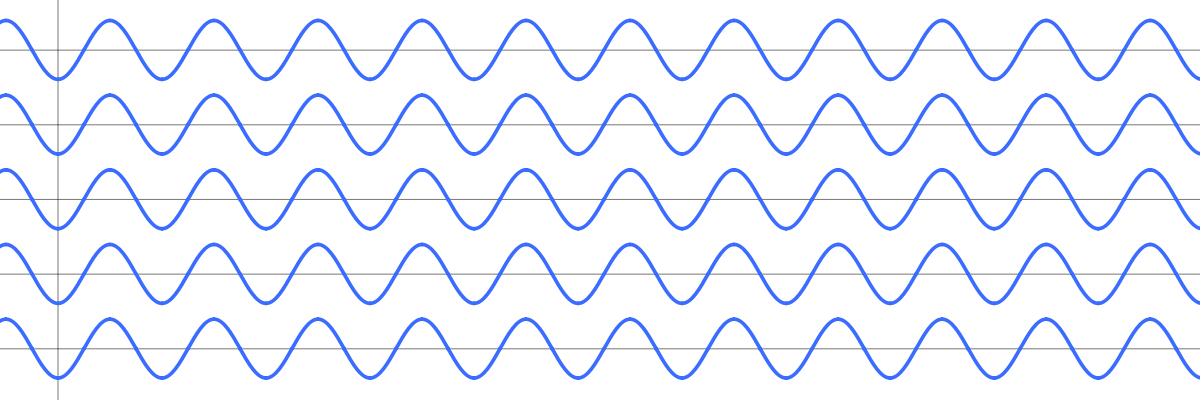
\includegraphics[width=.66\linewidth]{gfx/in-phase-waves.png}}
        \caption{Example of in-phase waves.}
        \label{fig:in-phase-waves}
\end{figure}

\begin{figure}[!h]
        \myfloatalign
        {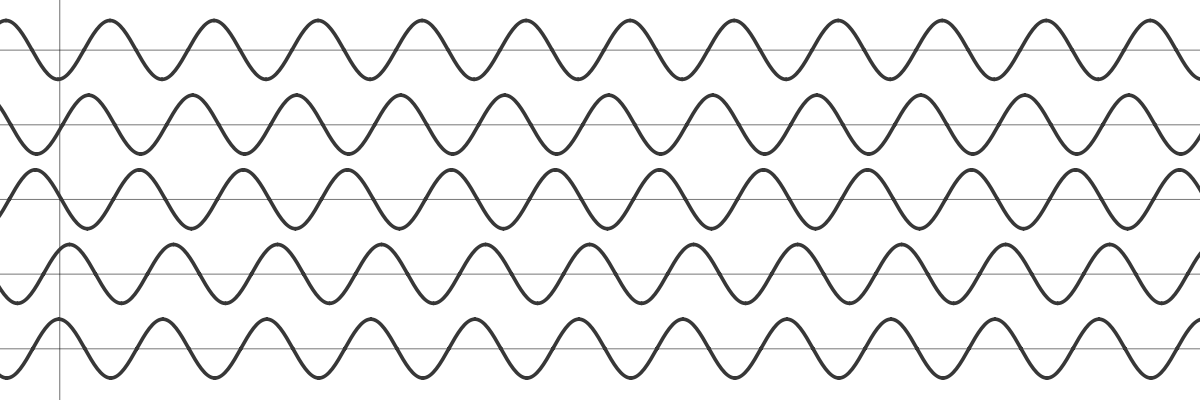
\includegraphics[width=.66\linewidth]{gfx/out-of-phase-waves.png}}
        \caption{Example of out-of-phase waves.}
        \label{fig:out-of-phase-waves}
\end{figure}

Another way of representing the audio information, which is more meaningful for human reading
or computer analysis is through short-term spectrum. Short-term spectra are obtained by applying
a Discrete Time Fourier transform to a windowed signal. At first, the signal is divided
into uniformly-spaced periods with a sliding window. For speech recognition, usually the window size is defined as 25 ms, 
with a frame shift of 10 ms, audio information is extracted every 10 ms with 15 ms of overlapping
among adjacent frames \cite{Huang2001}. \autoref{fig:audio-windowing} contains an example of a windowing process (in this case, 
with 50\% overlapping).

\begin{figure}[!h]
        \myfloatalign
        {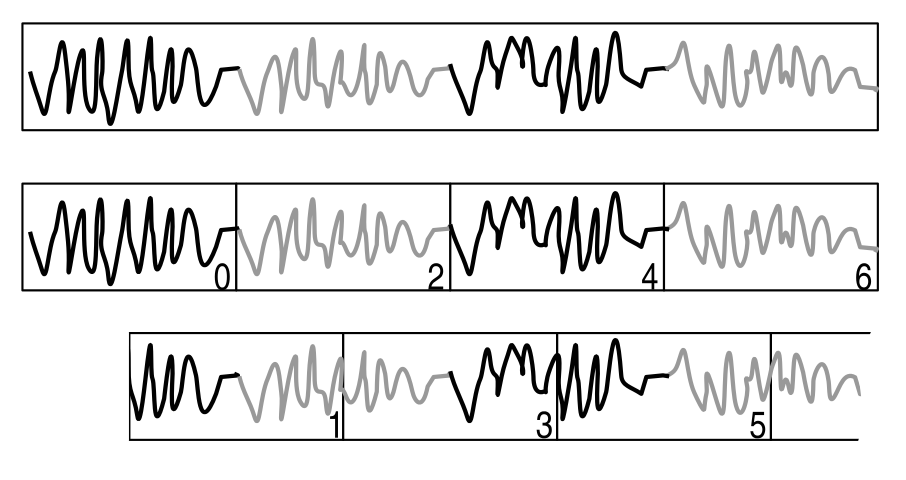
\includegraphics[width=.66\linewidth]{gfx/audio-windowing.png}}
        \caption{Illustration of an original audio recording (the upper waveform) divided into two
offset sequences of analysis windows (two lower waveforms) with 50\% overlapping frames \cite{McLoughlin2009}}
        \label{fig:audio-windowing}
\end{figure}

These windows values are based on two assuptions: (i) that within 25 ms the signal is stationary, i.e.
the phonatory system is not moving; (ii) that at least a period of each relevant speech frequency will 
be captured by this window
this windows, that is no relevant are 

After windowing the signal a Fourier transform is applied into each window so as to obtain
a series of frequency spectra, i.e. a series of representation of the signal in the frequency domain instead of the time domain. As can be noticed in \autoref{fig:audio-windowing}, since the frame shift is smaller than the window size, the windowing process extracts many redundant information. The intention for doing this will be made afterwards, when we give further details of the Fourier transform. Such transform is based on the Fourier theorem, which states that any periodic waveform can be approximated as closely as desired as the sum of a series of pure sine waves. In other words, the Fourier transform is able to analyse a short-term of the signal, containing a complex wave, and to output which are and what is the amplitude of the pure tones which form this complex wave.

Feature extraction must then be performed in stored audio files in order to extract relevant information from the waveform and discard redundant or unwanted signal characteristics. As already mentioned before, the two most traditional techniques for speech feature extraction, over the past decades, have been the \ac{MFCC} \cite{Davis1980} and the \ac{PLP} \cite{Hermansky1990}. Both parameterization methods are based on the short-term spectrum of speech. For speech recognition purposes, \ac{MFCC} features usually show better performance when compared to \ac{PLP}, for this reason in this thesis we are only going to present \ac{MFCC} features \cite{Muller2001, Mporas2007}.

\section{MFCC Features}

\ac{MFCC} is a type of speech parameterization is the result of a cosine transform of the logarithm of the short-term energy spectrum expressed over a mel scale \cite{Davis1980}. \ac{MFCC} features tries to reduce the feature dimensionality of a sound Fourier spectrum, by applying some concepts of Psychoacoustics and Psychophysics in order to the extract a vector with relevant values from the spectrum. The aim is to represent speech data in a compressed format, by eliminating information which are not pertinent to the phonetic analysis and to enhance the aspects of the signal which contribute to the detection of phonetic differences \cite{Davis1980}.

From Psychoacoustics, \ac{MFCC}s use the notion that humans do not perceive frequency through a linear scale, but through a scale which resembles to be linear-spaced in frequencies below 1000 Hz and logarithmic in frequecies above 1000 Hz\footnote{This is not entirely true. As shown by \citeauthor{Umesh1999}~\cite{Umesh1999}, in fact, there are no two distinguishable regions in terms of statistical significance. But the idea that we perceive low frequencies better than high ones still hold.}, the so-called mel scale (named after \emph{mel}ody). The scale is based on experiments with simple tones in which individuals are required to separat frequency values into four equal intervals or to adjust the frequency of a stimulus to be half as high as another reference tone \cite{Huang2001}. The reference point between mel scale and a linear frequency scale is 1000 mels, which correspond to a 1000 Hz tone, 40 dB above the absolute threshold of hearing. Since it was first introduced by \citeauthor{Stevens1937}~\cite{Stevens1937}, the scale has been revisited many times \cite{Umesh1999}, but a common formulation, according to \citeauthor{Huang2001}~\cite{Huang2001} is:
\begin{equation}
 M(f) = 1125*ln(1 + f / 700)
\end{equation}
where $f$ is the input frequency in Hz. The scale is plotted \autoref{fig:mel-scale}.
\begin{figure}[!ht]
        \myfloatalign
        {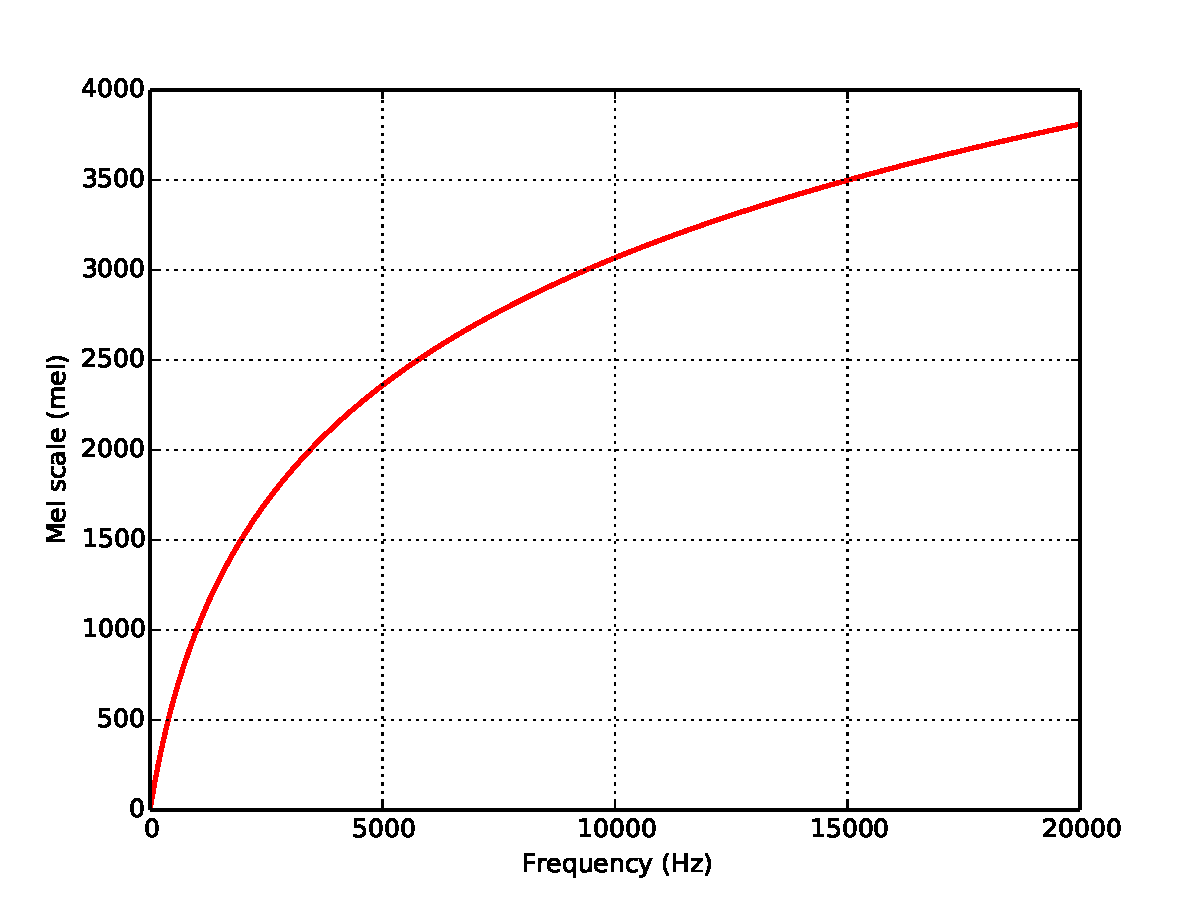
\includegraphics[width=1.\linewidth]{gfx/mel-scale.pdf}}
        \caption{Mel scale versus a linear frequency scale.}\label{fig:mel-scale}
\end{figure}

and also of the physics of speech, such as the fact that human like the these systems often have well defined overtones that are harmonic -- which is why the MFCCs use the FFT of the FFT)


\section{Dealing with Noisy Data}

One of the central problems in \ac{ASR} is how to deal with noisy audio data. It is long known that the performance of 
speech recognition systems greatly degrate when the environmental or the recording conditions are not controlled, 
thus allowing unwanted residual sounds to appear in the signal. In acoustics, any type of sound that is not the one
you are willing to analyze is considered noise. As a result from this, in speech recognition, the hiss of a fan, 
the buzz that a computer cooler makes, car horns on the street and so on are all regarded as noise. Even someone's voice
can be regarded as noise. Consider, for instance, that you are trying to recognize John's speech in an application, 
however Mary is close to him talking on the phone, to the extent that traces of her voice are added to the signal. In this
scenario, Mary's voice is actually noisy data, since it is undesirable for the given purpose. 


\section{Types of Speech Recognition Systems} 
Errem omnium ea per, pro \ac{UML} congue populo ornatus cu, ex qui
dicant nemore melius. No pri diam iriure euismod. Graecis eleifend
appellantur quo id. Id corpora inimicus nam, facer nonummy ne pro,
kasd repudiandae ei mei. Mea menandri mediocrem dissentiet cu, ex
nominati imperdiet nec, sea odio duis vocent ei. Tempor everti
appareat cu ius, ridens audiam an qui, aliquid admodum conceptam ne
qui. Vis ea melius nostrum, mel alienum euripidis eu.

\section{The Architecture of a Large Vocabulary Continuous Speech Recognition System} 
Non vices medical da. Se qui peano distinguer demonstrate, personas
internet in nos. Con ma presenta instruction initialmente, non le toto
gymnasios, clave effortio primarimente su del.\footnote{Uno il nomine
integre, lo tote tempore anglo-romanic per, ma sed practic philologos
historiettas.}